\newpage

\section*{Referencias}
\textbf{Básico: }
		\begin{itemize}
			\item \textit{Problema 1} tomado de OPM 2017-2018 Pre-olimpiadas 5ano problema 2. 
			\item \textit{Problema 2} tomado de OPM 2017-2018 Pre-olimpiadas 5ano problema 3.
			\item \textit{Problema 3} tomado de OPM 2017-2018 $2\degree$ eliminatoria, Junior problema 1.
			\item \textit{Problema 4} tomado de OPM 2017-2018 $2\degree$ eliminatoria, Junior problema 3.
		\end{itemize}
	
\textbf{Medio: }
\begin{itemize}
	\item \textit{Problema 1} tomado de OPM 2017-2018 $2\degree$ eliminatoria, Junior problema 3.
	\item \textit{Problema 2} tomado de OPM 2017-2018 $2\degree$ eliminatoria, Junior problema 4.
	\item \textit{Problema 3} tomado de OPM 2017-2018 $2\degree$ eliminatoria, Categoria A problema 1.
	\item \textit{Problema 4} tomado de OPM 2017-2018 $2\degree$ eliminatoria, Categoria A problema 4.
\end{itemize}

\textbf{Avanzado: }
\begin{itemize}
	\item \textit{Problema 1} tomado de OPM 2017-2018 $2\degree$ eliminatoria, Categoria A problema 3.
	\item	\textit{Problema 2} tomado de OPM 2017-2018 $2\degree$ eliminatoria, Categoria B problema 1.
	\item	\textit{Problema 4} tomado de OPM 2017-2018 $2\degree$ eliminatoria, Categoria B problema 2.
	\item	\textit{Problema 5} tomado de OPM 2016-2017 Final día 1, Categoria B problema 1.
\end{itemize}



%------------------------------------------------------------------------------------------------------------   
%----------------------------------                        BASICO                       ---------------------------------- 
%------------------------------------------------------------------------------------------------------------ 
\newpage
\section{Nivel Básico}\label{BASICO_2020_13_junio}
\begin{center}
	\fbox{\fbox{\parbox{6in}{\centering
				\textbf{Tiempo mínimo: } 2 horas y 30 minutos.\\
				\textbf{Tiempo máximo: } 4 horas.\\	
				\textbf{Procedimientos: }Cada problema debe estar resuelto por escrito, en forma detallada, todos los pasos seguidos para su resolución deben estar bien explicados. Se le brindarán unas hojas grapadas, en la \textit{parte de enfrente} de cada hoja debe estar la solución de los problemas, la \textit{parte posterior} no se leerá pero la pueden usar como borrador de los problemas\\
				\textbf{Puntaje máximo: }250 puntos.
	}}}
\end{center}

\begin{enumerate}
\item \textbf{50 puntos}. José tenía un terreno rectangular del cuál vendió una parte rectangular mas pequeña, quedandose solamente con un terreno de área $68m^2$, las medidas se muestran en la figura. El señor José pretende comprar una red para cercar su terreno. Sabiendo que el metro de red cuesta $50$ pesos, cuánto tendrá que gastar José para cercar su terreno?
		\begin{figure}[H]
			\centering
			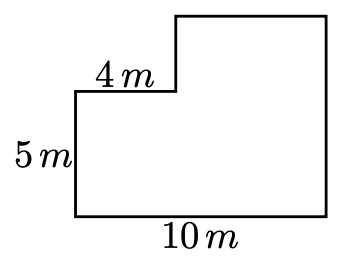
\includegraphics[width=0.4\linewidth]{2020_06_13/imgs/basic_p1}
			%\caption{}
			\label{basicp1}
		\end{figure}

\item \textbf{50 puntos}. Andrés tiene un trompo y quiere pintar los tres triángulos que tiene en su forma usando los colores amarillo, azul y rojo. Si Andrés quiere poder pintar regiones diferentes del mismo color, de cuántas maneras en total puede pintar su trompo?
		\begin{figure}[H]
			\centering
			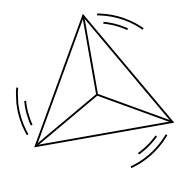
\includegraphics[width=0.2\linewidth]{2020_06_13/imgs/basic_p2}
			%\caption{}
			\label{basicp2}
		\end{figure}


\item \hspace{1cm}
	\begin{enumerate}[label=\Alph*)]
	\item \textbf{25 puntos}. Paulo es dueño de un terreno que está compuesto de tres cuadrados y tres trapecios. El área de cada cuadrado se muestra en la figura. Cuánto vale el lote sombreado sabiendo que cada $m^2$ vale 1 millón de pesos?
			\begin{figure}[H]
				\centering
				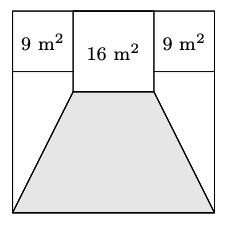
\includegraphics[width=0.4\linewidth]{2020_06_13/imgs/basic_p3_a}
				%\caption{}
				\label{basicp3a}
			\end{figure}
		
	\item \textbf{25 puntos}. Considere la siguiente lista de afirmaciones:
			\begin{enumerate}
			\item En esta lista hay exactamente una afirmación falsa.
			\item En esta lista hay exactamente dos afirmaciones falsas.
			\item En esta lista hay exactamente tres afirmaciones falsas.
			\item En esta lista hay exactamente cuatro afirmaciones falsas.			
			\end{enumerate}
			Cuál de las afirmaciones es verdadera? o ninguna es verdadera? 
			
	\item \textbf{25 puntos}. En cuántos ceros termina el número $8^7\times 25^5$?
	
	\item \textbf{25 puntos}. Un número de tres dígitos se dice que es \textit{cuadriñado} si es multiplo de cuatro y todos los números que se obtienen al desordenar sus dígitos también son múltiplos de cuatro. Por ejemplo, 408 es \textit{cuadriñado} porque 408, 084, 048, 840 y 804 son todos múltiplos de cuatro. Cuántos números \textit{cuadriñados existen}?
	\end{enumerate}

\item \textbf{50 puntos}. En un triángulo $CDE$, el punto $A$ está en $CD$ de forma que la distancia de $A$ a $C$ es $4cm$ y de $A$ a $D$ $8cm$. El punto $B$ está en $CE$ a $6cm$ de $C$ y $2cm$ de $E$. Si el área del triángulo $ABC$ es $3{cm}^2$, cuánto mide el área del triángulo $CDE$?


\end{enumerate}

%------------------------------------------------------------------------------------------------------------   
%----------------------------------                        MEDIO                       ---------------------------------- 
%------------------------------------------------------------------------------------------------------------ 

\newpage
\section{Nivel Medio}\label{MEDIO_2020_13_junio}

\begin{center}
	\fbox{\fbox{\parbox{6in}{\centering
				\textbf{Tiempo mínimo: } 2 horas y 30 minutos.\\
				\textbf{Tiempo máximo: } 4 horas.\\	
				\textbf{Procedimientos: }Cada problema debe estar resuelto por escrito, en forma detallada, todos los pasos seguidos para su resolución deben estar bien explicados. Se le brindarán unas hojas grapadas, en la \textit{parte de enfrente} de cada hoja debe estar la solución de los problemas, la \textit{parte posterior} no se leerá pero la pueden usar como borrador de los problemas\\
				\textbf{Puntaje máximo: }250 puntos.
	}}}
\end{center}

\begin{enumerate}
\item \textbf{50 puntos}. En un triángulo $CDE$, el punto $A$ está en $CD$ de forma que la distancia de $A$ a $C$ es $4cm$ y de $A$ a $D$ $8cm$. El punto $B$ está en $CE$ a $6cm$ de $C$ y $2cm$ de $E$. Si el área del triángulo $ABC$ es $3{cm}^2$, cuánto mide el área del triángulo $CDE$?

\item \textbf{50 puntos}. Siete amigos se sientan en una mesa a comer. De cuántas formas podemos escoger un grupo, por con lo menos una persona, de forma que no hayan dos personas que hayan estado sentadas al lado en la comida?

\item \hspace{1cm}
		\begin{enumerate}[label=\Alph*)]
			\item \textbf{25 puntos}. Paulo es dueño de un terreno que está compuesto de siete divisiones rectangulares como muestra la figura. El área algunas divisiones se muestra en la figura. Cuánto es el área del terreno de Paulo?
			\begin{figure}[H]
				\centering
				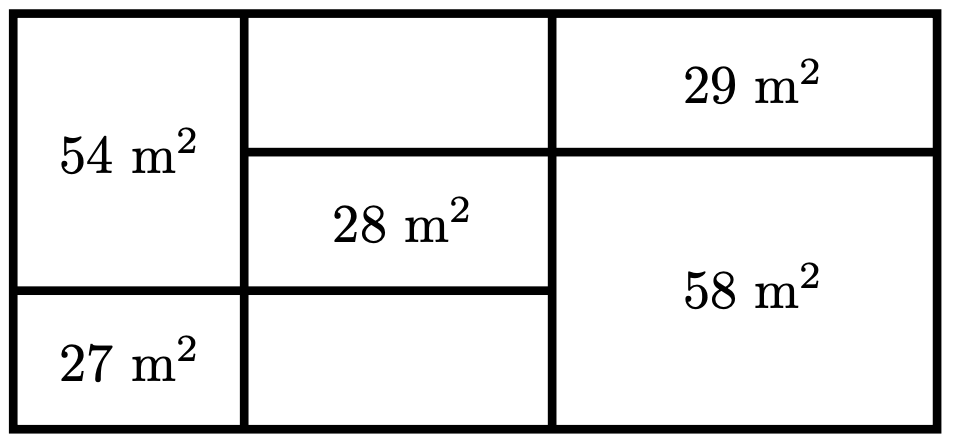
\includegraphics[width=0.4\linewidth]{2020_06_13/imgs/medio_p3_a}
				%\caption{}
				\label{medio_p3_a}
			\end{figure}
			
			\item \textbf{25 puntos}. En cuántos ceros termina el número $8^7\times 25^5$?
			
			\item \textbf{25 puntos}.  Juan nació entre 1989 y 1999 y solo sabe que una de las siguientes afirmaciones es falsa: ``Juan nació en un año par", ``Juan nació en un año múltiplo de 5", ``Juan nació en un año divisible por 3". Cuánto es el número de intentos necesarios para saber con certeza el año de nacimiento de Juan?
			
			\item \textbf{25 puntos}. Un número de tres dígitos se dice que es \textit{cuadriñado} si es multiplo de cuatro y todos los números que se obtienen al desordenar sus dígitos también son múltiplos de cuatro. Por ejemplo, 408 es \textit{cuadriñado} porque 408, 084, 048, 840 y 804 son todos múltiplos de cuatro. Cuántos números \textit{cuadriñados existen}?
		\end{enumerate}

\item \textbf{50 puntos}. En un juego de dardos, un jugador puede obtener 7 o 11 puntos en cada lanzamiento. La puntuacion de cada jugador es la suma de los puntos obtenidos en sus lanzamientos. Cuántos múltiplos de 5 son imposibles de obtener como puntuación en este juego, si no hay un límite de número de lanzamientos?
\end{enumerate}

%------------------------------------------------------------------------------------------------------------   
%----------------------------------                        AVANZADO                       ---------------------------------- 
%------------------------------------------------------------------------------------------------------------ 
\newpage
\section{Nivel Avanzado}\label{AVANZADO_2020_13_junio}

\begin{center}
	\fbox{\fbox{\parbox{6in}{\centering
				\textbf{Tiempo mínimo: } 2 horas y 30 minutos.\\
				\textbf{Tiempo máximo: } 4 horas.\\	
				\textbf{Procedimientos: }Cada problema debe estar resuelto por escrito, en forma detallada, todos los pasos seguidos para su resolución deben estar bien explicados. Se le brindarán unas hojas grapadas, en la \textit{parte de enfrente} de cada hoja debe estar la solución de los problemas, la \textit{parte posterior} no se leerá pero la pueden usar como borrador de los problemas\\
				\textbf{Puntaje máximo: }250 puntos.
	}}}
\end{center}

\begin{enumerate}
	\item \textbf{50 puntos}. Para desbloquear su celular, Juan utiliza contraseñas de 4 dígitos diferentes de cero de forma que el primer dígito es la suma de los otros tres. Si Juan cambia la contraseña todos los días, luego de cuántos días Juan se verá obligado a repetir contraseña?
	
	\item \textbf{50 puntos}. Cuál es el mayor múltiplo de 3 que no puede ser escrito de la forma $7a+11b$, donde $a$ y $b$ son números naturales?
	
	\item \textbf{50 puntos}. Diez amigos se sientan en una mesa a comer. De cuántas formas podemos escoger un grupo, por con lo menos una persona, de forma que no hayan dos personas que hayan estado sentadas al lado en la comida?
	
	\item \textbf{50 puntos}. Sea $\triangle ABC$ de área 9 y $D,E$ y $F$ puntos en los lados $AB, BC$ y $AC$ respectivamente tales que $DE\parallel AC$ y $DF\parallel BC$. Sabiendo que el área de $\triangle DEB$ es cuatro veces el área de $\triangle AFD$, cuál es el área de $\triangle CFE$?	
			\begin{figure}[H]
				\centering
				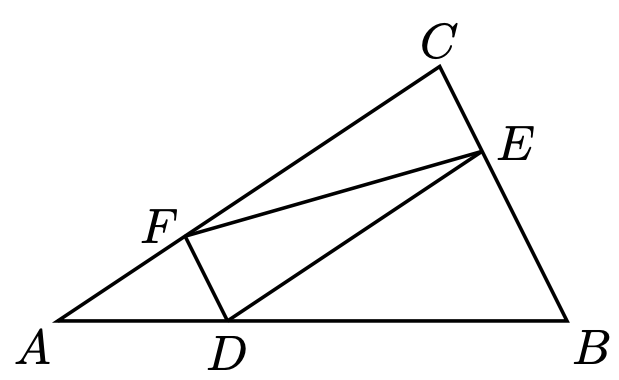
\includegraphics[width=0.45\linewidth]{2020_06_13/imgs/AV_P4}
				%\caption{}
				\label{avp4}
			\end{figure}
		
	\item \textbf{50 puntos}. Determinar todos los valores \textbf{enteros} de $n$ para los cuales el número
	\[\frac{14n+25}{2n+1}\]
	es un cuadrado perfecto.
	
\end{enumerate}